\documentclass[10pt, conference, compsocconf]{styles/IEEEtran}
\usepackage{cite}
\usepackage{balance}

\usepackage[pdftex]{graphicx}
\graphicspath{{figures/}}
\DeclareGraphicsExtensions{.pdf}

\usepackage[cmex10]{amsmath}
\interdisplaylinepenalty=2500
% \usepackage{algorithmic}
\usepackage[caption=false,font=footnotesize]{subfig}

\usepackage{url}
\usepackage[usenames,dvipsnames]{color}

% should be loaded last (but before algorithm*) -colored links and refs
\usepackage[colorlinks=true, citecolor=OliveGreen, linkcolor=BrickRed, urlcolor=MidnightBlue, final, pdftex]{hyperref}
\hypersetup
{
    pdfauthor={Authors},
    pdfsubject={Subject},
    pdftitle={Title},
    pdfkeywords={Keywords}
}

\usepackage{xspace}
\usepackage{algorithm}
\usepackage{algorithmic}

% Using watermark (this will mess up top/bottom margins)
\usepackage{styles/pdfdraftcopy}
\draftcolor{gray20}
\draftstring{
\begin{minipage}{17cm}
\begin{center}
\  DRAFT - \today\\Not approved for public release
\end{center}
\end{minipage}
}
\draftfontsize{36pt}

% custom commands
\newcommand{\etal}{{\em et al.}}
\newcommand{\naive}{na\"{\i}ve }
%\newcommand{\point}[1]{\vspace{2mm} \noindent\textbf{#1}}
\newcommand{\point}[1]{\noindent\textbf{#1}.}
\newcommand{\todo}[1]{\textbf{\color{red}[TODO: #1]}}
\renewcommand{\S}{Section~}

\title{Paper Title Placeholder}

\author{
\IEEEauthorblockN{Author1}
\IEEEauthorblockA{Institution1\\
Email1}
\and
\IEEEauthorblockN{Author2}
\IEEEauthorblockA{Institution1\\
Email2}
}

\begin{document}

\maketitle

\begin{abstract}
The scalability of the Tor Anonymity Network currently depends on volunteer relay operators for bandwidth. This is unsustainable. We present a method to compensate Tor relay operators and retain anonymity, without charging clients for access. Our solution relies on two novel concepts. First, we introduce \textit{TorCoin}, an ``altcoin'' that uses the BitCoin protocol to reward relays for contributing bandwidth. Relays ``mine'' TorCoins, then sell them for cash on any existing ``altcoin exchange.'' To verify that a given TorCoin represents actual bandwidth transferred, we introduce \textit{TorPath}, a decentralized protocol for assigning Tor circuits to clients, such that each is privately-addressable but publicly verifiable. [ADD TO THIS WHEN THE PAPER IS DONE]
\end{abstract}

% \begin{IEEEkeywords}
% anonymity; throttling; experimentation; Tor;
% \end{IEEEkeywords}
\section{Introduction}

\subsection{Launching a Secondary Tor Network}

We will build a system that enables deployment of a secondary, monetized Tor network. Independent communities can launch a private or public network that routes traffic over Tor. In exchange for supplying bandwidth, relay servers receive a special cryptocurrency called a TorCoin.

\subsection{TorCoin Mining}

Relay servers mine TorCoins proportionally to the bandwidth they supply. This mining is analagous to Bitcoin mining, except its proof-of-work scheme is bandwidth-intensive instead of CPU-intensive. As such, a TorCoin represents bandwidth that was pushed over some relay server, somewhere in the Tor network, at some point in time. Therefore, TorCoins have inherent value, because relay operators can trade them in for cash. 

\subsection{Exchanging TorCoins for Cash}

\subsubsection{TorCoins are Valuable to Both Clients and Outsiders}

A TorCoin has value to both clients and outsiders. For clients, a TorCoin has value because it represents bandwidth, which they demand and relays supply. For outsiders, TorCoin has value as an alternative cryptocurrency, also known as an “altcoin.” Increasingly, people are trading altcoins for arbitrage opportunities, money transferring vehicles, and speculative investment. So in this sense, TorCoin is similar to Namecoin, Zerocoin, and any other number of altcoins. 

Because a TorCoin has value to both clients and outsiders, relays have two counterparties for exchanging Torcoins.

\subsubsection{1. Charge clients for access to network}

One can imagine a scheme in which clients must pay a price, in traditional currency (or even Bitcoin), to access the network. Some mechanism then transfers the traditional currency to the relays, in exchange for Torcoins, which the client can use to connect to the network. That is, any client connecting to the network must pay some number of TorCoins. 

In this scenario, we have an open question: What happens to the Torcoins that the clients pay to the network? Relays already received cash for mining them and then selling them to clients via the exchange, so should they get the TorCoins back? This seems to be an ecomomic question, and a difficult one at that. So perhaps this next solution is a better one, as it's much more analagous to Bitcoin.

\subsubsection{2. Keep Tor free, sell TorCoins to AltCoin traders}

Because TorCoins have value outside of the relay-client relationship, they can also be exchanged outside of it. For example, relays who mine Torcoins could sell them on an Altcoin exchange, where traders set the price by trading amongst each other. Thus, relays can exchange Torcoins for cash without the client needing to pay for access to the network. Economically, this works because the relays create value by supplying anonymous bandwidth to clients, and then traders pay for that value as the supply of Torcoins grows.

(This leads us to an important question: Is the supply of Torcoins finite? Much of the appeal of Bitcoins and Altcoins is their finite money supplies. But if Torcoins have a finite money supply, then eventually no more can be mined. Then there is no more incentive for relays to supply bandwidth. So, we have a catch-22. We need to always incentivize relays to provide bandwidth, but Altcoin traders prefer currencies with finite money supplies. One possible solution to this is to reset the money supply every time it reaches its limit -- or even to launch a new Altcoin each time.)
\input{sections/model}
\input{sections/experiments}
\section{Related Work} \label{rel}

PAR~\cite{raykova-pet2008}, XPay~\cite{wpes09-xpay}, Gold Star~, BRAIDS~\cite{ccs10-braids}, Tortoise~, onions for sale~\cite{johnson2013onions}.

On the economics of anonymity~\cite{Acquisti03onthe}, one-to-n scrip systems~\cite{humbert2011-scrip}.

LIRA~\cite{jansen2013lira}is a lightweight system providing “performance incentives for users to contribute bandwidth to the Tor network.” It uses coins, similar to “in game currency,” to distribute payment. LIRA uses coins which have a tunable probability of being right, and clients can guess lottery tickets with probability, p of being right. 

Eigenspeed~\cite{snader2009eigenspeed} is a peer-to-peer consensus building algorithm for monitoring bandwidth over a network, specifically implemented for Tor. Unfortunately it requires a central authority for computing Principal Component Analysis operations. While we believe these operations could be decentralized, we are not interested in extending Eigenspeed. Instead, we exploit properties of the Bitcoin protocol to allow for bandwidth monitoring that is sufficient to generate payment tickets. However, as mentioned before, Eigenspeed could act as a secondary system to monitor relays and clients that seem to be producing more TorCoins than would be warranted by their speed.  
\section{Conclusions} \label{conc}

We have introduced TorPath, a novel scheme to assign paths to Tor
clients securely and anonymously.
TorPath motivated by the need to verifiably mine TorCoins, a
a BitCoin variant based on measured bandwidth over the Tor network.
The TorCoin protocol is robust to malicious relays and clients
colluding to mint TorCoins without transferring bandwidth.

\com{	This is a very minor optimization,
	not worth mentioning if it's the only "Future Work" listed. -baf
Further work could investigate the use of cryptographic accumulators for circuit
signatures, which could reduce the packet overhead during bandwidth-measurement
and make the protocol more efficient.
}

\subsection*{Acknowledgments}

This material is based upon work supported by the Defense Advanced Research
Agency (DARPA) and SPAWAR Systems Center Pacific, Contract No. N66001-11-C-4018.
This work was supported by the Office of Naval Research.



%\point{Acknowledgments}
% \section*{Acknowledgments}
% We thank the anonymous reviewers for their feedback and suggestions.

% trigger a \newpage just before the given reference
% number - used to balance the columns on the last page
% adjust value as needed - may need to be readjusted if
% the document is modified later
%\IEEEtriggeratref{22}
% The "triggered" command can be changed if desired:
%\IEEEtriggercmd{\enlargethispage{-5in}}
 
\newcommand{\BIBdecl}{\setlength{\itemsep}{0\baselineskip plus 0.1\baselineskip minus 0.1\baselineskip}}
\balance
{\footnotesize 
\bibliographystyle{styles/IEEEtran}
\bibliography{references}
}

\nocite{*}
 
%\clearpage
%\appendix
%\appendixpage
\section*{Appendices}

\section{Performance Rewards with Differentiated Services}

We now describe how the differentiated services
architecture~\cite{blake1998architecture} can be used to improve the control
over traffic priority in Tor, as previously outlined by
Jansen~\cite{jansenphdthesis}. More specifically, the proportional
differentiation model~\cite{dovrolis1999case} allows for predictable (i.e.,
consistent as load increases) and controllable (i.e., adjustable differentiation) performance between N traffic
classes. The model allows for the configuration of a differentiation parameter
$p_i$ for each class $i$, and enforces the proportional priority of a traffic
quality metric $q$ between all pairs of classes $i$ and $j$ for measurement
timescale $\sigma$ as:
\begin{equation}
\forall i \in [N], \forall j \in [N]: \frac{q_i \left( t, t + \sigma \right)}{q_j \left( t, t + \sigma \right)} = \frac{p_i}{p_j}
\end{equation}
where $p_1 < ... < p_N$ and $p_i/p_j$ defines the quality proportion between
classes $i$ and $j$. The model is well defined when there is enough
traffic in each class to allow a work-conserving scheduler to meet the desired
proportions.

Dovrolis \etal design a scheduler under the proportional differentiation model
using a queuing delay metric~\cite{dovrolis2002proportional}, which in our case
corresponds to Tor cell waiting times. For class $i$, the quality metric $q_i$
combines the queuing delay $D_i(t)$ of the longest waiting cell with the
long-term average delay $\delta_i(t)$  of all previously scheduled cells at time $t$:
\begin{equation}
q_i(t) = D_i(t) \cdot f + \delta_i(t) \cdot (1-f)
\end{equation}
where $f$ is an adjustable fraction that tunes the schedulers ability to react
to short term spikes in delay. When a scheduling decision is to be made at time $t$,
the longest waiting cell from the class with the maximum priority
$P(t) = q(t)/p(t)$ is chosen and scheduled.


Todo - DRAFT NOTES:

This section will detail the economic model and present any lingering questions. There will be another diagram featuring multiple clients, a PSP, and multiple hosts. The diagram below will go into the software architecture section, under a section called ``system design'', followed by a sentence describing each component. Then we will go into detail on the ephemeral paths and TorCoin design, which are part of the TorCoin Minter. The TorCoin trader, wallet, and exchange are all necessary, but not novel in terms of design, so we will spend little time on those.

TODO: Add component to Client, ``TorCoin Minter'' (?)

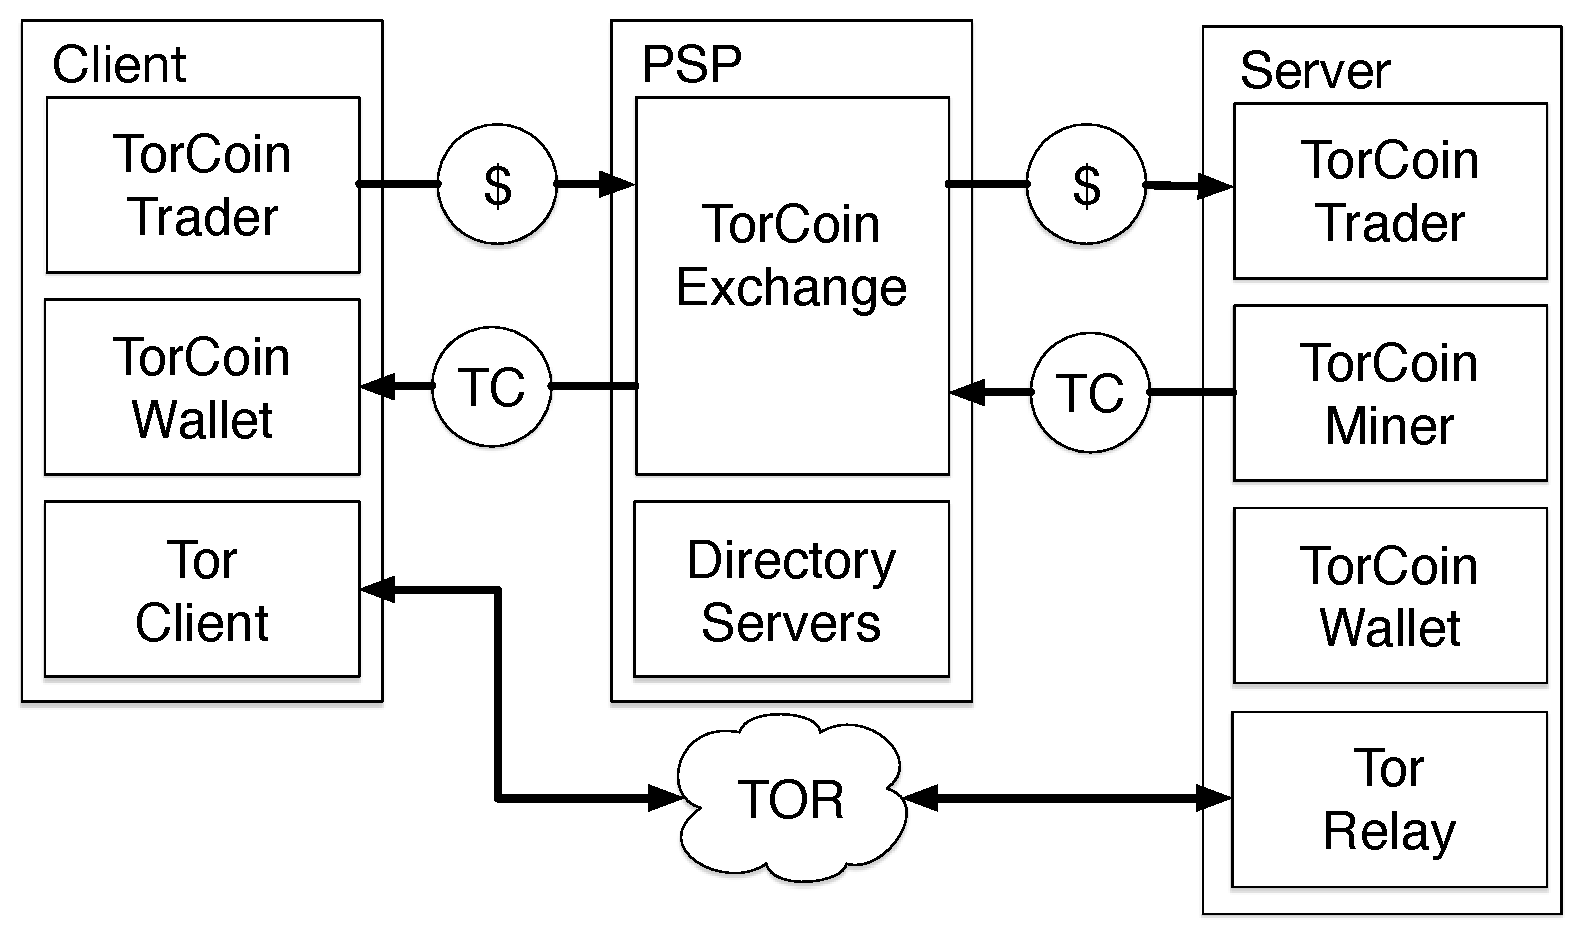
\includegraphics[scale=0.5]{figures/overview.pdf}

\end{document}
